\documentclass[11pt,twocolumn,oneside,openany,headings=optiontotoc,11pt,numbers=noenddot]{article}

\usepackage[a4paper]{geometry}
\usepackage[utf8]{inputenc}
\usepackage[T1]{fontenc}
\usepackage{lmodern}
\usepackage[ngerman]{babel}
\usepackage{ngerman}

\usepackage[onehalfspacing]{setspace}

\usepackage{fancyhdr}
\usepackage{fancybox}

\usepackage{rotating}
\usepackage{varwidth}

%Struktogramme
\usepackage[german,curves]{struktex}

\usepackage{pdflscape}
\usepackage{changepage}
\usepackage{graphicx}
\usepackage[bottom]{footmisc}
\usepackage{transparent}
\usepackage{graphbox}
\graphicspath{
	{Pics/PDFs/}
	{Pics/JPGs/}
	{Pics/PNGs/}
}
\usepackage{caption}
\usepackage{wrapfig}
\usepackage{marginnote}
\usepackage{tabularx}
\usepackage{dashrule}
\usepackage{soulutf8}
\usepackage{hhline}
%arydshln suppresses vertical lines in table
%\usepackage{arydshln}
\usepackage{multirow}
\usepackage{enumerate}
\usepackage[hidelinks]{hyperref}
\usepackage{listings}

\usepackage[table]{xcolor}
\usepackage{array}
\usepackage{enumitem,amssymb,amsmath}
\usepackage{interval}
\usepackage{cancel}
\usepackage{stmaryrd}
\usepackage{wasysym}
\usepackage{polynom}
\usepackage{diagbox}
\usepackage{dashrule}
\usepackage{framed}
\usepackage{mdframed}
\usepackage{karnaugh-map}
\usepackage{pdfpages}

\usepackage{blindtext}

\usepackage{eso-pic}

\usepackage{amssymb}
\usepackage{eurosym}

\usepackage[pages=some]{background}
\pagestyle{headings}
\renewcommand{\headrulewidth}{0.2pt}
\renewcommand{\footrulewidth}{0.2pt}
\newcommand*{\underdownarrow}[2]{\ensuremath{\underset{\overset{\Big\downarrow}{#2}}{#1}}}
\setlength{\fboxsep}{5pt}
\newcommand{\explainBelow}[3]{\underbrace{#1}_{\parbox{\widthof{#3}}{\footnotesize\raggedright #2}}}
\newcommand{\explainAbove}[3]{\overbrace{#1}^{\parbox{\widthof{#3}}{\footnotesize\raggedright #2}}}
\newcommand\footnoteref[1]{\protected@xdef\@thefnmark{\ref{#1}}\@footnotemark}


% Codestyle defined
\definecolor{codegreen}{rgb}{0,0.6,0}
\definecolor{codegray}{rgb}{0.5,0.5,0.5}
\definecolor{codepurple}{rgb}{0.58,0,0.82}
\definecolor{backcolour}{rgb}{0.95,0.95,0.92}
\definecolor{deepgreen}{rgb}{0,0.5,0}
\definecolor{darkblue}{rgb}{0,0,0.65}
\definecolor{mauve}{rgb}{0.40, 0.19,0.28}
\colorlet{exceptioncolour}{yellow!50!red}
\colorlet{commandcolour}{blue!60!black}
\colorlet{numpycolour}{blue!60!green}
\colorlet{specmethodcolour}{violet}

%Neue Spaltendefinition
\newcolumntype{L}[1]{>{\raggedright\let\newline\\\arraybackslash\hspace{0pt}}m{#1}}
\newcolumntype{M}{>{\centering\arraybackslash}X}
\newcommand{\cmnt}[1]{\ignorespaces}
%Textausrichtung ändern
\newcommand\tabrotate[1]{\rotatebox{90}{\raggedright#1\hspace{\tabcolsep}}}

%Intervall-Konfig
\intervalconfig {
	soft open fences
}

%Bash
\lstdefinestyle{BashInputStyle}{
	language=bash,
	basicstyle=\small\sffamily,
	backgroundcolor=\color{backcolour},
	columns=fullflexible,
	backgroundcolor=\color{backcolour},
	breaklines=true,
}
%Java
\lstdefinestyle{JavaInputStyle}{
	language=Java,
	backgroundcolor=\color{backcolour},
	aboveskip=1mm,
	belowskip=1mm,
	showstringspaces=false,
	columns=flexible,
	basicstyle={\footnotesize\ttfamily},
	numberstyle={\tiny},
	numbers=none,
	keywordstyle=\color{purple},,
	commentstyle=\color{deepgreen},
	stringstyle=\color{blue},
	emph={out},
	emphstyle=\color{darkblue},
	emph={[2]rand},
	emphstyle=[2]\color{specmethodcolour},
	breaklines=true,
	breakatwhitespace=true,
	tabsize=2,
}
%Python
\lstdefinestyle{PythonInputStyle}{
	language=Python,
	alsoletter={1234567890},
	aboveskip=1ex,
	basicstyle=\footnotesize,
	breaklines=true,
	breakatwhitespace= true,
	backgroundcolor=\color{backcolour},
	commentstyle=\color{red},
	otherkeywords={\ , \}, \{, \&,\|},
	emph={and,break,class,continue,def,yield,del,elif,else,%
		except,exec,finally,for,from,global,if,import,in,%
		lambda,not,or,pass,print,raise,return,try,while,assert},
	emphstyle=\color{exceptioncolour},
	emph={[2]True,False,None,min},
	emphstyle=[2]\color{specmethodcolour},
	emph={[3]object,type,isinstance,copy,deepcopy,zip,enumerate,reversed,list,len,dict,tuple,xrange,append,execfile,real,imag,reduce,str,repr},
	emphstyle=[3]\color{commandcolour},
	emph={[4]ode, fsolve, sqrt, exp, sin, cos, arccos, pi,  array, norm, solve, dot, arange, , isscalar, max, sum, flatten, shape, reshape, find, any, all, abs, plot, linspace, legend, quad, polyval,polyfit, hstack, concatenate,vstack,column_stack,empty,zeros,ones,rand,vander,grid,pcolor,eig,eigs,eigvals,svd,qr,tan,det,logspace,roll,mean,cumsum,cumprod,diff,vectorize,lstsq,cla,eye,xlabel,ylabel,squeeze},
	emphstyle=[4]\color{numpycolour},
	emph={[5]__init__,__add__,__mul__,__div__,__sub__,__call__,__getitem__,__setitem__,__eq__,__ne__,__nonzero__,__rmul__,__radd__,__repr__,__str__,__get__,__truediv__,__pow__,__name__,__future__,__all__},
	emphstyle=[5]\color{specmethodcolour},
	emph={[6]assert,range,yield},
	emphstyle=[6]\color{specmethodcolour}\bfseries,
	emph={[7]Exception,NameError,IndexError,SyntaxError,TypeError,ValueError,OverflowError,ZeroDivisionError,KeyboardInterrupt},
	emphstyle=[7]\color{specmethodcolour}\bfseries,
	emph={[8]taster,send,sendMail,capture,check,noMsg,go,move,switch,humTem,ventilate,buzz},
	emphstyle=[8]\color{blue},
	keywordstyle=\color{blue}\bfseries,
	rulecolor=\color{black!40},
	showstringspaces=false,
	stringstyle=\color{deepgreen}
}

\lstset{literate=%
	{Ö}{{\"O}}1
	{Ä}{{\"A}}1
	{Ü}{{\"U}}1
	{ß}{{\ss}}1
	{ü}{{\"u}}1
	{ä}{{\"a}}1
	{ö}{{\"o}}1
}

% Neue Klassenarbeits-Umgebung
\newenvironment{worksheet}[3]
% Begin-Bereich
{
	\newpage
	\sffamily
	\setcounter{page}{1}
	\ClearShipoutPicture
	\AddToShipoutPicture{
		\put(55,761){{
				\mbox{\parbox{385\unitlength}{\tiny \color{codegray}BBS I Mainz, #1 \newline #2
						\newline #3
					}
				}
			}
		}
		\put(455,761){{
				\mbox{\hspace{0.3cm}
\includegraphics[width=0.2\textwidth]{../../logo.pdf}}
			}
		}
	}
}
% End-Bereich
{
	\clearpage
	\ClearShipoutPicture
}

\setlength{\columnsep}{3em}
\setlength{\columnseprule}{0.5pt}

\geometry{left=1.50cm,right=1.50cm,top=2.50cm,bottom=1.00cm,includeheadfoot}
\pagenumbering{gobble}
\pagestyle{empty}

\begin{document}
	\begin{worksheet}{BS FI}{1. Lehrjahr, LF 4 - Einfache IT-Systeme}{Digitaltechnik}
		\section*{Die Konstruktion des Karnaugh-Diagramms}
		Betrachten wir uns die Funktionstabelle für eine boolesche Funktion \(f_1\) mit zwei Eingangsvariablen. Da es nur vier Ausgangszustände (\(2^2\)) gibt, benötigen wir im zugehörigen Karnaugh-Diagramm nur ein (2 x 2) Diagramm.\\
		\begin{karnaugh-map}[2][2][1][$x_0$][$x_1$]
			
		\end{karnaugh-map}\\
		Ergänzen wir unsere Funktion nun auf drei Eingangsvariablen, müssen wir das Diagramm zunächst etwas anpassen. Um beim übertragen aus der Funktionstabelle in das Diagramm nicht viel nachdenken zu müssen, ziehen wir die Variable \(x_1\) nach oben, ergänzen somit das Diagramm um zwei Spalten und reduzieren es zunächst auf eine Spalte.\\
		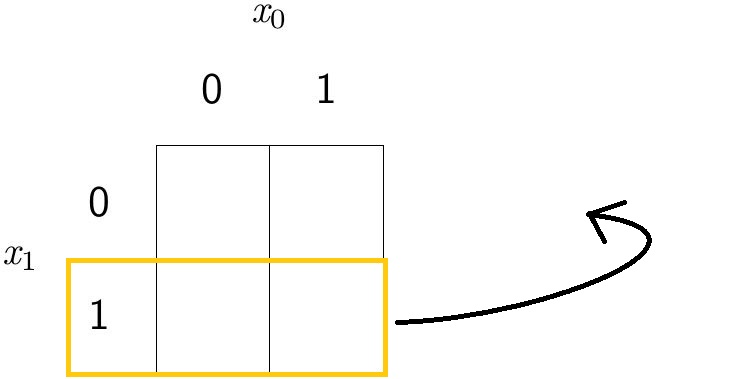
\includegraphics[width=0.4\textwidth]{../99_Bilder/190219_2x2zu1x4.jpg}\\
		So ergibt sich dann das nachfolgende Layout.\\
		\begin{minipage}{0.2\textwidth}
			\renewcommand{\arraystretch}{1.4}
			\begin{tabularx}{1.1\textwidth}{|L{0.5cm}|L{0.5cm}|L{0.5cm}|L{0.5cm}|}
				\multicolumn{4}{c}{$x_1x_0$}\\
				\multicolumn{1}{c}{00} & \multicolumn{1}{c}{01} & \multicolumn{1}{c}{11} & \multicolumn{1}{c}{10}\\
				\hline
				& & & \\
				\hline
			\end{tabularx}\\
			\par\noindent
		\end{minipage}
		\hfill
		\begin{minipage}{0.2\textwidth}
			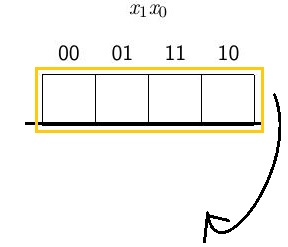
\includegraphics[width=0.98\textwidth]{../99_Bilder/190219_1x4zu2x4.jpg}
		\end{minipage}\\
		Es fehlt noch die dritte Eingangsvariable. Diese hat entsprechend zwei Zeilen. Wir weisen der ersten Zeile den Zustand \(0\) zu und erweitern um eine weitere Zeile, die den Zustand \(1\) erhält.\\
		\newpage
		Damit ergibt sich für \underline{drei Eingabevariablen}: (2 x 4)\\
		\par\noindent
		\begin{karnaugh-map}[4][2][1][$x_1x_0$][$x_2$]
			
		\end{karnaugh-map}
		\par\noindent
		Möchten wir nun um eine vierte Eingangsvariable erweitern, nutzen wir die untere Kante des Diagramms als Spiegelachse.\\
		\par\noindent
		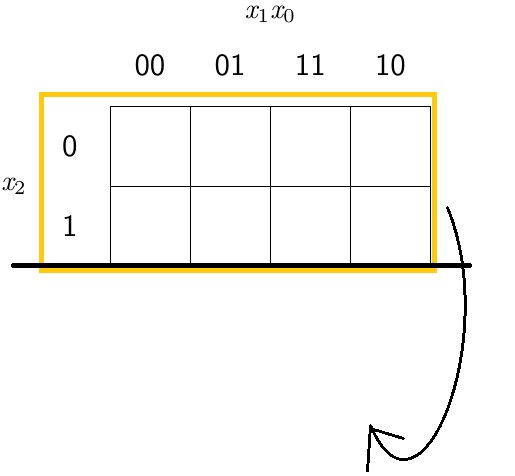
\includegraphics[width=0.28\textwidth]{../99_Bilder/190219_2x4zu4x4.jpg}\\
		Damit ergibt sich zunächst das folgende Diagramm:\\
		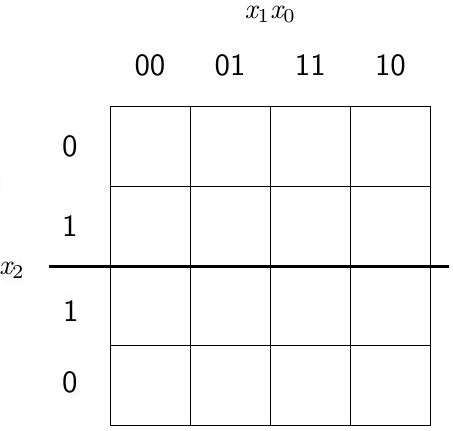
\includegraphics[width=0.28\textwidth]{../99_Bilder/190219_4x4_3.jpg}\\
		Um nun die vierte Eingangsvariable betrachten zu können, müssen wir diese entsprechend anbringen.\\
		Bei der Zeilen- bzw. Spaltenzählung ist zu beachten, dass sich von einer zur nächsten Zeile bzw. Spalte jeweils nur \underline{\textbf{eine}} Variable ändern darf.\\
		Innerhalb der \textit{K-Map} werden die Zellen mit einer \(1\) befüllt, deren Belegung bei der Funktion auch eine \(1\) als Ausgabe haben.
		\section*{Vereinfachen mit der K-Map - Überdeckung der Einsen}
		Bei der Vereinfachung von Schaltfunktionen ist unser Ziel, so wenig Schaltelemente (\textit{NOT, AND} bzw. \textit{OR}) wie möglich zu nutzen.\\
		Um die aus der Funktionstabelle aufgestellte Funktion zu minimieren, versuchen wir im Karnaugh-Diagramm so viele \(1\)en wie möglich\footnote{Die Anzahl muss immer einer \underline{2er Potenz} entsprechen.} zusammenzufassen. Dabei sind folgende Überdeckungen bzw. Zusammenfassungen zulässig:
		\begin{itemize}
			\item[+] zwei nebeneinander/übereinander liegende \(1\)en\\
			\begin{karnaugh-map}[4][4][1][$x_1x_0$][$x_3x_2$]
				\minterms{0,1,7,15}
				\implicant{0}{1}
				\implicant{7}{15}
			\end{karnaugh-map}
			\item[+] vier zusammenhängende \(1\)en\\
			\begin{karnaugh-map}[4][4][1][$x_1x_0$][$x_3x_2$]
				\minterms{0,1,4,5,9,11,13,15}
				\implicant{0}{5}
				\implicant{13}{11}
			\end{karnaugh-map}
			\item[+] zwei bzw. vier über die Außenkanten nebeneinander/übereinander liegende \(1\)en
			\begin{karnaugh-map}[4][4][1][$x_1x_0$][$x_3x_2$]
				\minterms{0,1,2,4,6,9}
				\implicantedge{1}{1}{9}{9}
				\implicantedge{0}{4}{2}{6}
			\end{karnaugh-map}
			\item[+] zwei oder vier in den Ecken befindliche \(1\)en
		\end{itemize}
		\begin{karnaugh-map}[4][4][1][$x_1x_0$][$x_3x_2$]
			\minterms{0,2,8,10}
			\implicantedge{0}{0}{2}{2}
			\implicantedge{8}{8}{10}{10}
		\end{karnaugh-map}\\
		bzw.\\
		\begin{karnaugh-map}[4][4][1][$x_1x_0$][$x_3x_2$]
			\minterms{0,2,8,10}
			\implicantcorner
		\end{karnaugh-map}
	\end{worksheet}
\end{document}